\chapter{The Soviet economy}
\label{ch:sovieteconomy}

\section{The argument about incentives, and how it was settled}

Between 1963 and 1965 the Cuban leadership held, in public and in print, one of
the more serious debates in the history of socialist economics. On one side Che
Guevara, then Minister of Industries, argued for a budgetary finance system in
which enterprises were departments of a single national firm with no accounts of
their own, transfers between them were not sales, and workers were motivated by
moral incentives --- emulation, voluntary labour, the formation of a new kind of
person --- rather than by pay. On the other, Carlos Rafael Rodr\'iguez and the
economists of the old communist party argued for self-finance on the Soviet
model of the period, in which enterprises kept books, faced prices, and paid
bonuses.

The debate was conducted with more intellectual honesty than the subject
usually receives, and Guevara's side of it is worth reading; his objection to
using capitalist categories to build socialism is coherent, and his warning
that material incentives would reproduce the mentality they were meant to serve
turned out to be, in the Soviet case, prescient. He was also wrong about
everything operational. A system without prices cannot tell which of two
processes is cheaper, a system without enterprise accounts cannot locate a
loss, and a system in which effort is rewarded by a certificate produces, after
the first enthusiasm, exactly the effort a certificate is worth.

The debate was not settled by argument. Guevara left the government in 1965;
his approach was applied maximally through the late 1960s, culminating in the
1968 abolition of small business and in an economy where money had almost
stopped functioning --- rents, utilities, local telephone calls, burials,
sporting events and school meals were free, wages were paid but there was
progressively less to buy with them, and absenteeism reached levels the state
could not control. Then, after 1970, the whole apparatus was replaced wholesale
with the Soviet system Rodr\'iguez had argued for.

\section{Ten million tons}

The pivot was a sugar harvest.

Having failed at rapid industrialisation in the early 1960s --- an attempt to
substitute imports across the board, which foundered on the absence of inputs,
spares and anyone who had run a factory --- Cuba returned to sugar as the source
of accumulation, and in 1968 the leadership committed publicly to a harvest of
ten million tons in 1970, a figure roughly a third above anything the country
had ever produced. The commitment was made in Castro's characteristic register:
as a matter of national honour, with a date, in a speech.

The mobilisation to meet it was total. Factories closed and their workers went
to the cane. Students, soldiers, office staff, foreign volunteers went to the
cane. Transport, fuel, spares and management attention were pulled out of every
other sector. The harvest ran into July, wrecking the following season's
planting. The country produced 8.5 million tons, the largest harvest in Cuban
history before or since, and the effort broke the rest of the economy: output
fell across manufacturing, transport and construction, the cane fields were
damaged for years, and the mills had been run past maintenance.

On 26 July 1970 Castro made a speech admitting the failure in unusually direct
terms, taking personal responsibility, and offering to resign. The crowd
refused, as everyone in the square and on the platform knew it would. What
followed the speech, however, was a real change of system, and it went in the
opposite direction to the one the speech implied. Cuba stopped trying to invent
its own socialism and adopted the Soviet one.

\section{Institutionalisation, 1972--1976}

Cuba joined the Council for Mutual Economic Assistance, Comecon, in July 1972.
It adopted five-year plans, a central planning board, and in 1976 the SDPE,
the System of Direction and Planning of the Economy, a close copy of the Soviet
enterprise model with cost accounting, profit indicators and bonuses. The First
Congress of the Communist Party met in 1975, sixteen years after the
revolution. A new constitution was approved by referendum in 1976, replacing
the 1940 constitution as amended; it defined the party as the leading force of
society and state, and created \emph{Poder Popular}, a system of municipal,
provincial and national assemblies elected from the base, with direct secret
competitive election at municipal level and indirect selection above it. The
provinces were redrawn from six into fourteen. A civil and criminal code
followed, and a family code.

The period 1971--1985 was, in ordinary economic terms, the best Cuba has had.
Growth was solid, consumption improved, the housing programme delivered
through the \emph{microbrigadas} --- work teams seconded from their enterprises
to build apartment blocks, with the flats allocated back to the enterprise ---
and the social indicators of Chapter~\ref{ch:socialstate} reached their peaks.
Cubans who are nostalgic for the revolution are, almost always, nostalgic for
these fourteen years specifically.

\section{What was actually paying for it}

The arithmetic underneath is the single most important thing to understand
about Cuba, because everything in Part II is the consequence of its
disappearance.

Cuba's trade with the Soviet Union was not trade at world prices. Under the
long-term sugar protocols the USSR bought Cuban sugar at a price fixed well
above the world market --- in some years of the early 1980s at four or five
times it --- and supplied crude oil at a price fixed well below it. Nickel and
citrus had similar arrangements. Payment ran through a bilateral clearing
account in transferable rubles rather than in convertible currency, so that
Cuba's persistent deficit accumulated as a debt that never had to be settled in
anything the Soviet Union could spend elsewhere.

On top of the price terms there was a second mechanism, and it is the one that
is usually left out. Cuba was allocated more Soviet oil than it consumed, and
was permitted to re-export the surplus for hard currency. By the mid-1980s this
re-export was one of the largest single sources of Cuba's convertible-currency
earnings --- in some years the largest, ahead of sugar.\unv{} Cuba was, in
effect, being handed a petroleum rent by a country that had oil and wanted an
ally in the Caribbean.

The magnitudes are not small and they are not in serious dispute. In 1987 the
Soviet Union paid Cuba the equivalent of about 42 US cents a pound for sugar
against a world price of under 7 cents --- more than six times the market ---
and a CIA assessment earlier in the decade found a comparable ratio on a volume
of 3.2 million tonnes. Converting the whole relationship into dollars is harder,
because it depends on what rate one applies to transferable rubles, which is the
problem the note on sources described. But the standard estimates put the
combined inflow at around 23 per cent of Cuban output over 1985--88, reaching
something over four billion dollars in a single year \citep{mesalago2000}.\unv{}
Roughly a quarter of national income, from one patron, sustained for over a
decade. By 1990 the accumulated debt to the USSR
stood at something over twenty billion transferable rubles, a figure Russia
would later claim in dollars and eventually, in 2014, write off ninety per cent
of.

Alongside it Cuba had borrowed in hard currency from Western banks and
governments in the 1970s, when sugar prices were briefly high and Cuban credit
was good. When they fell, it could not pay: Cuba suspended payments on its
convertible-currency debt in 1986 and has been in default to the Paris Club
essentially ever since. That default is thirty-nine years old in 2026 and it is
the reason Cuba cannot borrow, which is the reason it cannot invest, which is a
constraint Chapter~\ref{ch:money} has to solve before anything else in Part III
is financeable.

\begin{figure}[t]
\centering
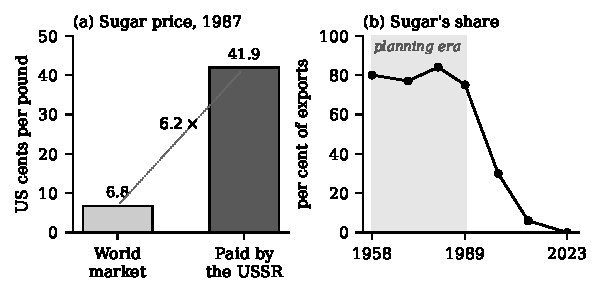
\includegraphics[width=\linewidth]{figs/comecon}
\caption{The subsidy, and what it bought. (a)~The mechanism: in 1987 the Soviet
Union paid more than six times the world price for Cuban sugar, and supplied oil
below it. (b)~The result: sugar's share of Cuban merchandise exports barely
moved across thirty years of planning, the highest investment rate in Latin
America and a Comecon membership organised around international specialisation
--- and then collapsed when the buyer went. A guaranteed price removes the only
signal that tells a producer to become good at something else. Panel~(a) is two
measured values rather than a series, because the year-by-year price data is not
reliably public and drawing a line through two points would invent the shape;
the post-1989 values in~(b) are estimates, flagged in \texttt{verify.md}. Generated by
\texttt{figs/comecon.py}.}
\label{fig:comecon}
\end{figure}

\section{The failure that mattered: no diversification}

Here is the fact that indicts the whole period, and Fig.~\ref{fig:comecon}(b) is its picture. In 1958, sugar was about four
fifths of Cuban exports. In 1989, after thirty years of planning, three decades
of the highest investment rates in Latin America, a Comecon membership
explicitly organised around international specialisation, and the best-educated
workforce in the region, sugar was still about three quarters of Cuban
exports \citep{onei,mesalago2000}.\unv{}

Everything else was small. Nickel, from the Moa and Nicaro deposits, was
second. Tobacco, citrus, fish and rum followed. The industrial base built in
the 1970s was assembly and import substitution for the domestic market, ran on
Soviet inputs, and could not export outside Comecon because its costs and
quality were set by a market that did not test either. A pharmaceutical and
biotechnology capability was started in the early 1980s --- of which much more
in Chapter~\ref{ch:life}, because it is the one exception and the one asset ---
but it was a decade from products in 1989.

The reason for the failure is not mysterious and it is not the embargo. A
protected market at guaranteed prices removes the only signal that tells a
producer to become better at something else. Cuba had, for eighteen years, the
sweetest terms of trade any small country has ever been offered, and it used
them to remain a sugar economy with a very good school system. That is the
central economic lesson of Part I, and Chapter~\ref{ch:premises} states it as a
constraint on the design: \emph{a guaranteed buyer at a political price is not
a market, and an economy built on one does not develop.} It applied to the
American sugar quota before 1959 and it applied to the Soviet protocols after,
and Chapter~\ref{ch:venezuela} will show it applying a third time to
Venezuelan oil.

\section{Rectification, 1986}

In 1980, under pressure from food shortages, Cuba opened free farmers' markets
where cooperatives and private farmers could sell surplus above their state
quota at whatever price the market bore. They worked: food appeared. They also
produced visible inequality --- intermediaries, some farmers doing very well,
prices the poorest could not pay --- and complaints about profiteering.

In 1986 Castro launched the Rectification of Errors and Negative Tendencies. It
closed the farmers' markets. It banned private house construction for sale and
much private artisanal work. It curtailed the enterprise bonus system of the
SDPE, denounced material incentives, revived voluntary labour and the
contingent brigades, and rehabilitated Guevara's economic thinking explicitly
by name.

The timing is the point. In 1986 the Soviet Union was beginning perestroika.
Cuba responded to its patron's turn toward markets by turning away from them,
and it did so eighteen months before the terms of trade that made the choice
affordable began to disappear. Rectification is the clearest single instance of
the pattern this book will name in Chapter~\ref{ch:ledgerch} and that recurs
through Part II: \emph{Cuba liberalises under duress and re-centralises as soon
as the pressure lifts, and the re-centralisation always arrives just before it
is least affordable.}

\begin{ledger}{the Soviet economy, 1963--1989}
\emph{Achieved.} Fourteen years of solid growth and the highest living
standards the revolution has produced. A universal social state financed to
completion. Mass housing through the microbrigades. Full employment, in the
sense that everyone had a job. Institutional forms --- a constitution, a party
congress, elected municipal assemblies, codified law --- where before there had
been improvisation by speech. An education system whose output was, and remains,
the country's best asset. The founding of a biotechnology capability that would
outlive everything else here.

\emph{Cost.} Thirty years of accumulation that left the export basket where it
was in 1958, three quarters sugar, because guaranteed prices removed the reason
to change it. An economy structurally dependent on transfers running between a
fifth and a third of national income, from a single patron, with no plan for
their ending. A hard-currency default in 1986 that has locked the country out
of credit markets ever since. An enterprise system that could not calculate,
and a workforce whose pay had been decoupled from what it did. And a decision
in 1986 to reverse the one reform that had visibly worked, taken at the last
moment when reversing it was still survivable.
\end{ledger}
